\documentclass[11pt, a4paper]{article}
\input{preamble.tex}
\switchlang{en}
\begin{document}

\title{1989 "--- Aero trackball}
\date{}
\maketitle
\selectlanguage{english}
The Aero trackball presented in the figure \ref{fig:AeroPhoto} was introduced to the market by Taiwanese company ICA Technology in 1990 \cite{mouses4, mouses5}. Marketing materials \cite{mouses5} mention the trackball's ``advanced optomechanical technologies, dynamic resolution from 100 to 1000 dpi, typically set to 200 dpi'' (that is, apparently, software resolution scaling), and an ``improved electronic clock'' as part of the trackball.

\begin{figure}[h]
    \centering
    
\includegraphics[scale=0.7]{1990_aero_trackball/pic_30.jpg}
    \caption{Aero trackball}
    \label{fig:AeroPhoto}
\end{figure}

The trackball's body is designed in a futuristic 1980s style, with rectangular shapes and jagged edges that match the style. The main body is made of beige plastic. Three large gray buttons are located on the top of the body. The trackball keys, shown in the figure \ref{fig:AeroTopBottom} as the lower left and lower right keys, correspond to the left and middle mouse buttons, while the upper right key serves as the right mouse button. A ball, approximately 4.5 cm in diameter, is located in the center of the case. Finally, a digital clock is located in the upper left corner of the case.

On the underside, there are a ribbed sleeve protecting the cable from damage in place of it's exit from the case, a label with technical data, rubber feet to ensure the device remains stable on a desk, and a switch allowing to select the communication mode.

Apparently, the developers intended the trackball's size and shape to more or less match those of a typical computer keyboard. Because of this, and given the relatively small ball, the device is flat but quite bulky (fig. \ref{fig:AeroSize}).

\begin{figure}[h]
    \centering
    
\includegraphics[scale=0.7]{1990_aero_trackball/top_30.jpg}
    
\includegraphics[scale=0.7]{1990_aero_trackball/bottom_30.jpg}
    \caption{Aero trackball, top and bottom views}
    \label{fig:AeroTopBottom}
\end{figure}

ICA Technology designed the Aero trackball with the anatomy of a human hand in mind. Despite its futuristic, broken facet shape, the hand position on the body is quite comfortable (fig. \ref{fig:AeroHand}), and the large buttons enhance its usability even further. An obvious drawback of the trackball is the inability to remove the ball for cleaning without disassembling the body.

\begin{figure}[h]
    \centering
    
\includegraphics[scale=0.4]{1990_aero_trackball/size.jpg}
    \caption{Aero trackball on a graduated pad with a grid step of 1~cm}
    \label{fig:AeroSize}
\end{figure}

~

The switch on the bottom provides choices between the two-button Microsoft mouse (``MS'') and three-button Mouse Systems mouse (``PC'') protocols. The package includes a driver with installation and testing programs, as well as a program to creating and activating a user menu, allowing the Aero Trackball to be used for commands to the applications that do not support mouse. The package also includes a graphics editor for DOS.

\begin{figure}[h]
    \centering
    
\includegraphics[scale=0.41]{1990_aero_trackball/hand_30.jpg}
    \caption{Aero trackball with a human hand model}
    \label{fig:AeroHand}
\end{figure}

The disassembled trackball is shown in the figure \ref{fig:AeroInside}. The photo shows the optomechanical design fairly typical for the 1990s, as well as the electronic clock assembly, additionally secured to the upper part of body with paper adhesive tape for ease of assembly and not connected to either the computer or the trackball electronics unit.

\begin{figure}[h!]
    \centering
    
\includegraphics[scale=0.53]{1990_aero_trackball/inside_30.jpg}
    \caption{Aero trackball disassembled}
    \label{fig:AeroInside}
\end{figure}

The review presented in \cite{mouses4} delicately notes that the trackball's built-in clock has its own power source and is therefore independent of the computer. Therefore, the device's LCD display serves no other functions than displaying the current time and is not software-controlled. Also, given the impossibility of removing the clock without disassembling the device, replacing its power source (which is a battery, typical for small watches) was not a priority during the trackball's development.

Removing the clock from its case reveals that it was apparently originally intended for sale as a standalone device. At least, its case is equipped with a folding stand for placing it on a tabletop (fig. \ref{fig:AeroClock}). The time value can be adjusted in a manner standard for the 1970s electronic watch, with two buttons on its front panel.

\begin{figure}[h]
    \centering
    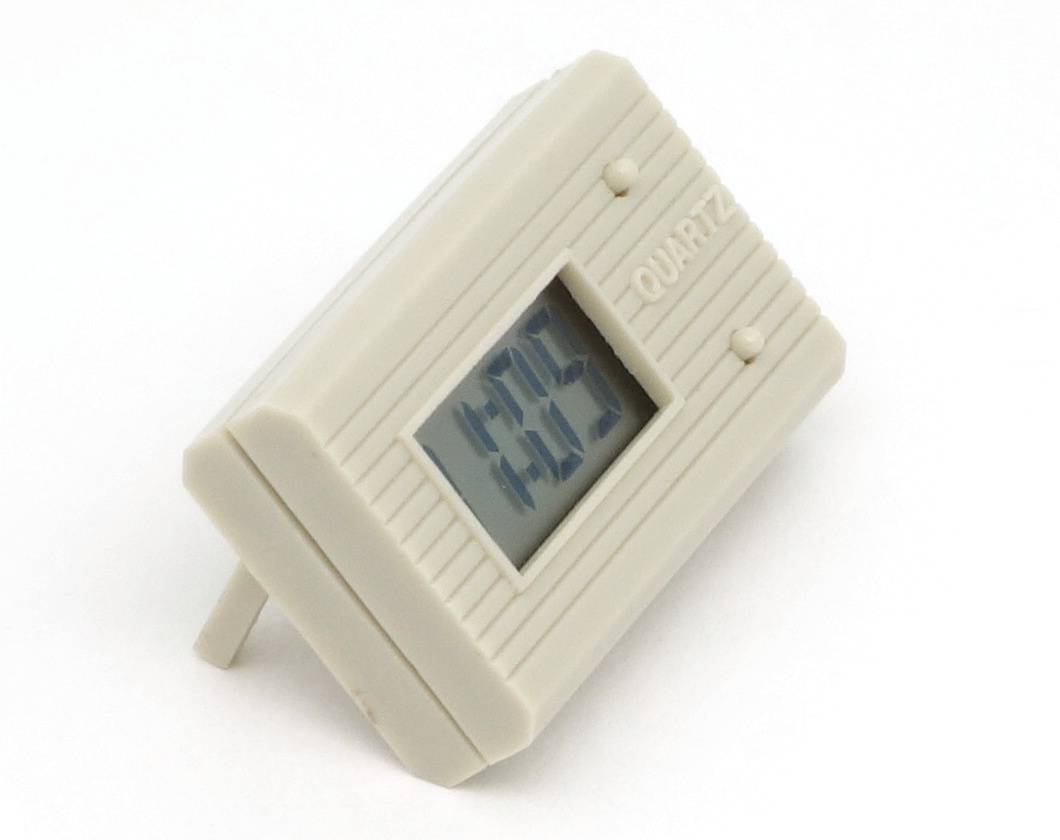
\includegraphics[scale=0.86]{1990_aero_trackball/clock_30.jpg}
    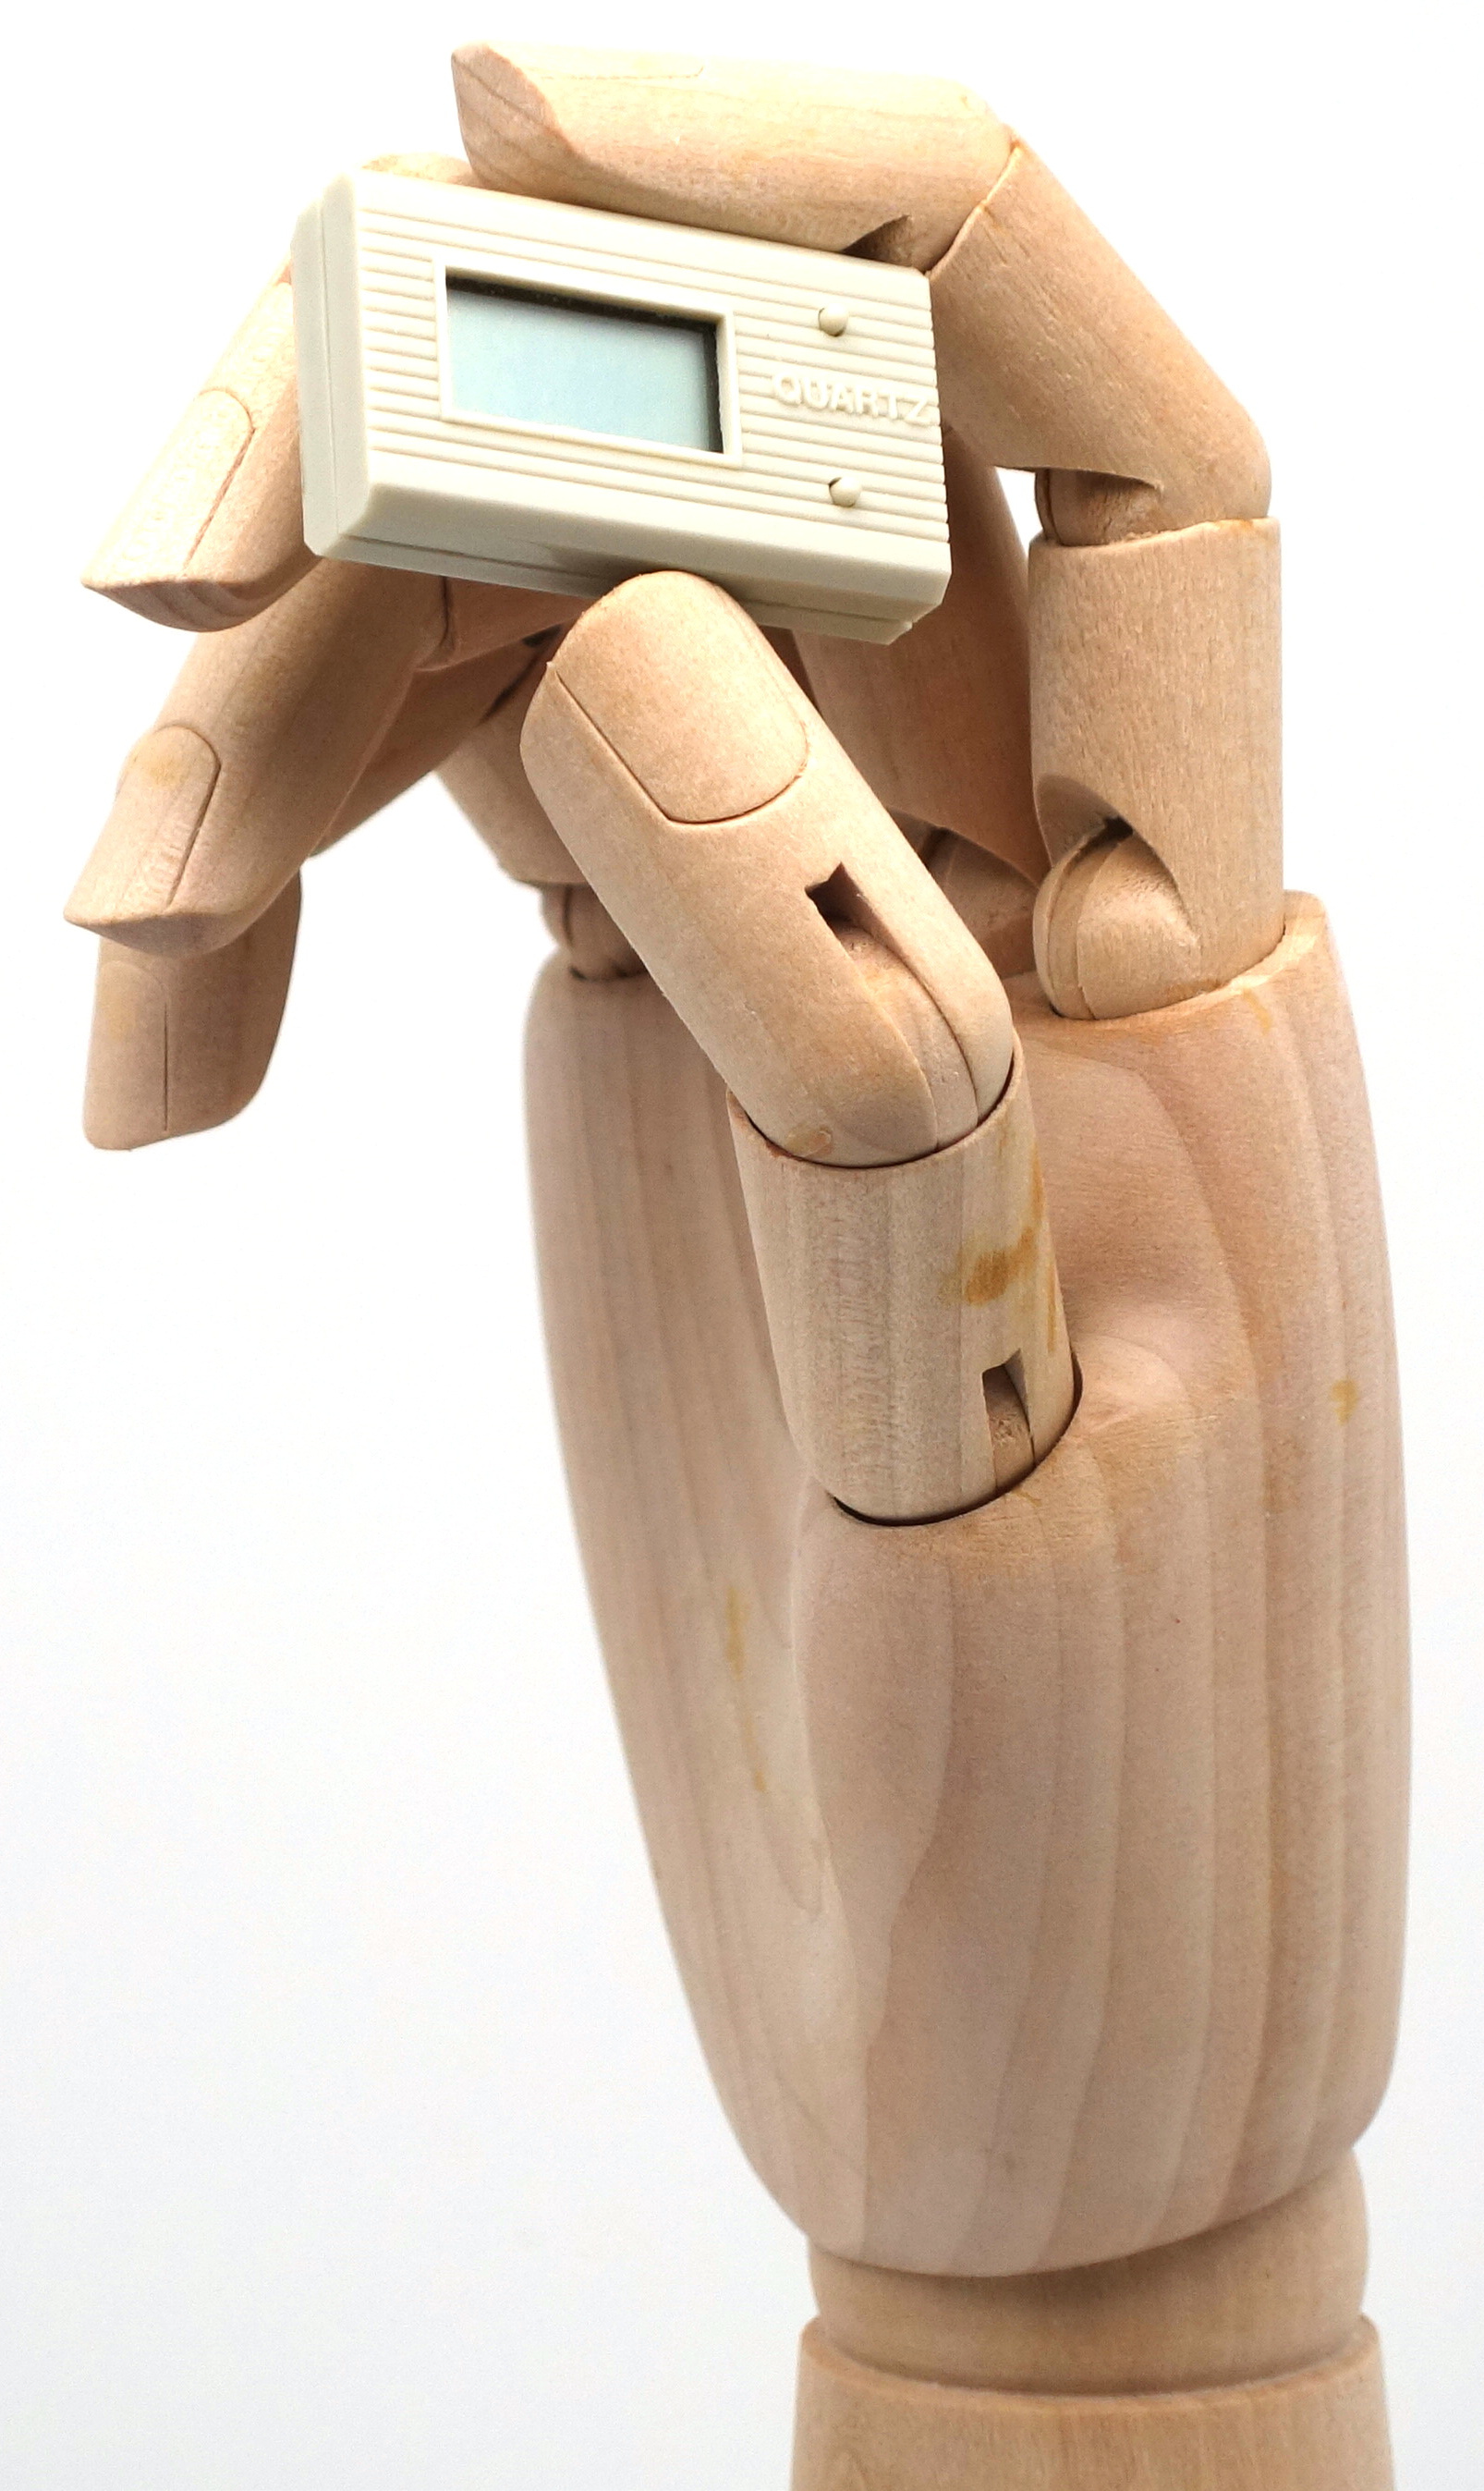
\includegraphics[scale=0.66]{1990_aero_trackball/hand_clock_30.jpg}
    \caption{The watch retrieved during the disassembly of the Aero Trackball}
    \label{fig:AeroPedal}
\end{figure}

\begin{thebibliography}{9}
	\bibitem {mouses4} Zmaga s cistim tusem // Moj Micro, No. 4, April 1991. P. 14--15. \url{https://archive.org/details/Moj_Micro_1991_04/page/n13/mode/2up}
	\bibitem {mouses5} Aero trackball reaches your fingers // BYTE, February 1991, P. 74. \url{https://archive.org/details/eu_BYTE-1991-02_OCR/page/n153/mode/2up}
\end{thebibliography}
\end{document} 
